\section{Creazione del server principale}

Il server principale è il componente con il compito 
di ricevere tutte le richieste dai client,
elaborarle e restituire le informazioni volute,
eventualmente a seguito di un'interrogazione verso la persistenza centrale.
Per poter essere in grado di rispondere a un numero sempre maggiore di utenti,
idealmente senza che questo impatti sul tempo di risposta o sulle performance in generale,
deve essere implementato in maniera tale da poter permettere un'esecuzione distribuita,
riducendo al minimo le dipendenze che possano minarne la duplicazione.\\
\\
Per soddisfare questo tipo di esigenza
esistono servizi definiti come Function as a Service (FaaS).
I FaaS sono servizi serverless,
ovvero la loro gestione hardware è completamente delegata al gestore del cloud;
il cui scopo è quello di duplicare ed eseguire il progetto,
suddiviso e implementato attraverso molteplici funzioni.
Ogni funzione consiste in un'unità indipendente di codice,
e in quanto tale crea la possibilità di essere eseguita 
in un ambiente di esecuzione unico per ogni richiesta.
Questa caratteristica, 
combinata con la virtualizzazione dell'ambiente di esecuzione,
consente una scalabilità potenzialmente illimitata.\\
\\
L'indipendenza della funzione dipende dalla relazione 
con le altre parti del progetto e dalla sua natura stateless.
L'esecuzione di una funzione infatti,
oltre a dover essere limitata rispetto a qualunque dipendenza logica che possa dover essere condivisa,
deve essere svincolata dalle informazioni sullo stato o sulla sessione.
Queste caratteristiche, per loro natura, 
non possono essere garantite dal servizio,
e sono quindi una responsabilità di chi deve svilupparle.\\
\\
Per assicurarne l'autonomia,
le funzioni dovranno essere implementate seguendo il principio di singola responsabilità.
Ogni Function adempirà un solo compito specifico,
creando una restrizione delle dipendenze e
garantendo il minimo utilizzo di risorse necessarie per rispondere alla richiesta.
Inoltre, viene così semplificata la creazione e la manutenzione del codice,
riducendo il controllo dell'esecuzione all'esito del tentativo di risoluzione del singolo problema.
\clearpage
\subsection{Individuazione del servizio adatto}

I gestori in cloud che offrono servizi FaaS sono limitati.
Escludendo i fornitori improntati allo sviluppo di applicazioni principalmente front-end,
i fornitori sul mercato con servizi testati e maturi sono
Amazon Web Services con AWS Lambda, 
Azure con Azure Functions e
Google Cloud Provider con Google Cloud Functions.
Tuttavia, queste tre soluzioni si assomigliano particolarmente.
Nonostante siano state tutte implementate usando una tecnologia proprietaria,
le proprietà computazionali, il supporto ai linguaggi e il costo risultano molto simili.\\
\\
Presentano tutti una granularità relativa
alla scalabilità delle richieste a livello di funzione,
ovvero permettono di duplicare il solo codice necessario per l'esecuzione della funzione richiesta.
Il supporto ai linguaggi è molto esteso,
ma offrono tutti comunque la possibilità di creare un runtime personalizzato,
di fatto supportando tutte le tecnologie.\\

\begin{longtable} {|P{3.5cm}|P{3.7cm}|P{3.7cm}|P{3.7cm}|}
    \hline
                                                    & \textbf{AWS Lambda}                                         & \textbf{Azure Functions} & \textbf{Google Cloud Functions} \\
    \hline
    \endhead
    Linguaggi supportati                            &
    Node.js, Python, Java, C\#, Go, PowerShell, Ruby, PHP
                                                    &
    Node.js, Python, Java, C\#, PowerShell, F\#, PHP
                                                    &
    Node.js, Python, Java, C\#, Go, F\#, Visual Basic                                                                                                                          \\
    \hline
    Runtime Personalizzato                          & Sì, tramite i custom deplyment packages o AWS Lambda Layers &
    Sì, grazie ai custom handlers                   &
    Sì, tramite immagini Docker personalizzate                                                                                                                                 \\
    \hline
    Massimo tempo di esecuzione                     &
    15 minuti                                       &
    Dai 10 ai 60 minuti, in base al piano di pagamento
                                                    &
    60 minuti per le richieste HTTP, 9 minuti per le richieste a eventi                                                                                                        \\
    \hline
    Massima memoria dedicata a funzione             &
    10 GB                                           &
    Da 1.5 GB a 14 GB in base al piano di pagamento &
    4 GB                                                                                                                                                                       \\
    \hline
    Tempo medio di attesa prima di essere spento    &
    Dai 5 ai 7 minuti                               &
    Tra i 20 e i 30 minuti                          &
    15 minuti                                                                                                                                                                  \\
    \hline
    Tempo medio di cold-startup                     &
    Generalmente sotto il secondo                   &
    Non oltre i 5 secondi                           &
    Da mezzo secondo a 2 secondi                                                                                                                                               \\
    \hline
    Orchestrazione                                  &
    Sì, tramite AWS Step Functions                  &
    Sì, tramite Durable Azure Functions             &
    Sì, tramite GCP workflow                                                                                                                                                   \\
    \hline
    \textbf{Costi}                                  &                                                             &                          &                                 \\
    \hline
    Richieste gratuite mensili                      &
    400.000 GB-seconds                              &
    400.000 GB-seconds                              &
    400.000 GB-seconds                                                                                                                                                         \\
    \hline
    Tempo di esecuzione gratuita al mese            &
    1 milione                                       &
    1 milione                                       &
    2 milioni                                                                                                                                                                  \\
    \hline
    Costo della richiesta al consumo                &
    \$0.20 per milione                              &
    \$0.20 per milione                              &
    \$0.40 per milione                                                                                                                                                         \\
    \hline
    Costo di esecuzione al consumo                  &
    \$0.000016 per GB-seconds                       &
    \$0.000016 per GB-seconds                       &
    \$0.0000125 per GB-seconds                                                                                                                                                 \\
    \hline
    Arrotondamento della durata                     &
    1 millisecondo                                  &
    1 millisecondo                                  &
    100 millisecondi                                                                                                                                                           \\
    \hline
    \caption{Caratteristiche delle principali FaaS}
\end{longtable}

La principale differenza tra queste soluzioni
risulta nel tempo necessario in caso di start up,
ma bisogna notare che,
oltre a essere solo una fase particolare del suo ciclo di vita,
dipende molto dal linguaggio di programmazione,
dalle dipendenze e dalla dimensione del progetto.
Viene inoltre mitigato dal tempo di attesa 
per il quale le istanze rimangono accese pronte a ricevere richieste e
dalla quantità degli utenti attivi che,
generando un flusso continuo di richieste,
contribuiscono a diminuire la frequenza dello spegnimento.\\
\\
Essendo le differenze tra un servizio e l'altro minime,
sia a livello di costi che di prestazioni,
ed essendo il progetto improntato su Azure,
la scelta della tecnologia su cui implementare il server principale
è ricaduta sulle Azure Functions.\\

\subsection{Scelte progettuali derivate dall'utilizzo delle Azure Functions}

L'utilizzo di un servizio FaaS
comporta un approccio particolare per la scrittura del codice.
A differenza di un programma normale,
dove l'esecuzione del programma è indipendente dalla ricezione di un evento,
nelle FaaS l'invocazione di un processo avviene esplicitamente a partire da un fattore esterno
(che sia una richiesta HTTP o il messaggio in una coda).
Non bisogna più preoccuparsi di come far interagire le parti dell'applicazione,
ma piuttosto di come rispondere nella maniera più efficiente possibile a tanti singoli problemi.
Ogni funzione dovrà essere implementata come entità autonoma rispetto al resto del sistema,
con l'unica responsabilità di rispondere a un solo incarico specifico.\\
\begin{wrapfigure}{r}{0.25\textwidth}
    \centering
    
\includegraphics[height=.12\textheight]{functions.png}
    Azure Functions
\end{wrapfigure}
La difficoltà principale del procedimento sussiste nell'individuare i singoli compiti
in cui suddividere l'applicazione.
Raramente una richiesta può essere soddisfatta in un unico passaggio,
e non è quindi automatico che a una Function corrisponda una sola parte di codice,
soprattutto in quanto alcune richieste potrebbero avere alcune parti in comune
(ad esempio, l'autenticazione è necessaria alla maggior parte delle richieste).
Nel caso in cui una richiesta si componga di più passaggi logici,
per poterli racchiudere in un'unica Function bisogna analizzarne la relazione.\\
\par
Innanzi tutto ogni passaggio deve essere implementato
sempre in maniera indipendente e stateless come richiesto alle Azure Function.
A questo punto è necessario però che tutti i passaggi siano in diretta successione,
e che il fallimento di uno solo di questi comporti il fallimento di tutta la funzione.
In caso contrario, è sconsigliato raggrupparle in un'unica funzione,
quanto piuttosto suddividerli in altre piccole funzioni
(con le stesse proprietà di cui sopra),
per poi coordinarle tramite l'utilizzo di un orchestratore o di code di eventi.\\
\\
L'orchestratore è una funzione che ha la caratteristica
di poterne invocare e controllare altre.
Consente di gestire efficacemente scenari
in cui è richiesta un'esecuzione particolare delle operazioni, sia essa sequenziale o parallela,
dove è necessario effettuare tentativi aggiuntivi in caso di errore o fallimento o
si richiede l'attesa del completamento di operazioni con un tempo di esecuzione prolungato.
Tuttavia, la natura stateless e l'accoppiamento debole tra orchestratore
e le Function in esecuzione causano un tempo di risposta delle richieste più elevato.\\
\\
Integrato all'interno delle Azure Functions,
Azure Durable Function consente la creazione di un orchestratore,
incaricato di gestire l'ordine, lo stato,
il ciclo di vita e le risposte delle varie Function coinvolte nell'elaborazione della richiesta,
mantenendo un'architettura indipendente e scalabile.\\
\\
Il coordinamento tramite code di eventi prevede 
invece l'invio di un evento al sistema
durante l'esecuzione della prima funzione,
nel momento in cui questa abbia terminato la sua responsabilità diretta
e possa delegare ulteriori procedimenti.
L'evento verrà aggiunto in coda,
per poi invocare una seconda funzione nel momento in cui sarà preso in carico.
Si consente così di separare logicamente le funzioni tra loro
senza introdurre ulteriori logiche e garantendo un tempo di risposta alla prima funzione minimo.
Questo approccio introduce però alcune problematiche.\\
\\
Disaccoppiando le due funzioni la prima
non ha conoscenza sull'esito della seconda,
ed è quindi necessario che la funzione invocata dalla coda
non svolga un compito essenziale
o che siano previste logiche di controllo,
rilancio o segnalazione dell'esito.
La possibilità che la stessa funzione
venga eseguita più volte con lo stesso messaggio
richiede che il suo comportamento sia idempotente,
ovvero che la sua eventuale esecuzione duplicata non impatti sul risultato finale.
Inoltre l'invocazione verrà così considerata come doppia,
andando a influire sui costi totali.\\
\\
Come linguaggio di programmazione per lo sviluppo delle Function è stato utilizzato C\#.
La consapevolezza che sia l'ambiente di sviluppo di C\#,
ovvero il framework .Net, sia la piattaforma Azure
siano entrambi sviluppati e mantenuti dalla stessa azienda, Microsoft,
garantisce elevati livelli di stabilità,
supporto e coordinamento delle tecnologie adottate.\\
\\
Azure Functions in ambiente .Net supporta due modelli di esecuzione e sviluppo:
in-process worker o isolated worker.
Il worker è il processo all'interno dell'applicativo che gestisce 
l'esecuzione delle funzioni in risposta alle richieste.
Nella modalità in-process,
il worker viene eseguito all'interno dello stesso processo 
dell'host che lo genera,
riducendo la quantità di allocazione delle risorse necessarie
ma condividendo l'ambiente di esecuzione.
Nel modello isolated invece
il worker esegue le funzioni in un secondo un processo,
garantendo maggiore isolamento e aumentando il controllo sulle funzioni.\\
\\
Inoltre, il modello isolated worker offre ulteriori vantaggi
grazie al maggiore supporto fornito.
Innanzi tutto esso prevede una maggiore compatibilità nel tempo,
grazie al più ampio numero di versioni del framework .Net a disposizione.
Il modello in-process, differentemente, 
è limitato alle sole versioni con supporto a lungo termine.
In secondo luogo il supporto per la creazione di middleware personalizzati
permette l'elaborazione di un codice intermedio 
tra la chiamata e l'esecuzione della funzione,
funzionalità invece non disponibile nel modello in-process.
Considerati questi vantaggi, 
le funzioni sono state sviluppate utilizzando il modello isolated worker
per garantire maggiore flessibilità, 
compatibilità e modularità dell'architettura.\\
\\
Lo sviluppo è stato condotto utilizzando Visual Studio Code,
programma open source sviluppato dalla stessa Microsoft per la creazione di codice.
Visual Studio Code permette l'integrazione con molteplici estensioni 
fornendo il supporto per la maggior parte delle tecnologie.
In particolare, grazie alle estensioni dedicate al provider Azure,
è possibile collegare il proprio ambiente di lavoro direttamente con i servizi in cloud.
Il legame così creato consente un aggiornamento immediato e intuitivo del codice,
gestito interamente dal programma.
\clearpage


\subsection{Implementazione della logica applicativa}
Per quanto ogni funzione ricopra un unico compito,
alcune parti della sua risoluzione possono essere condivise con altre.
Per questo motivo,
la logica applicativa è stata suddivisa 
in metodi che risolvono una specifica esigenza logica,
che saranno poi chiamati dalle funzioni quando necessario.
I metodi vengono quindi raggruppati in classi in base all'inerenza dei loro scopi,
concentrando il codice che condivide le stesse necessità e uniformando il suo stile.
Le dipendenze vengono così inizializzate un'unica volta a livello di classe,
creando un software più ordinato.\\
\begin{figure}[h!]
    \begin{center}
        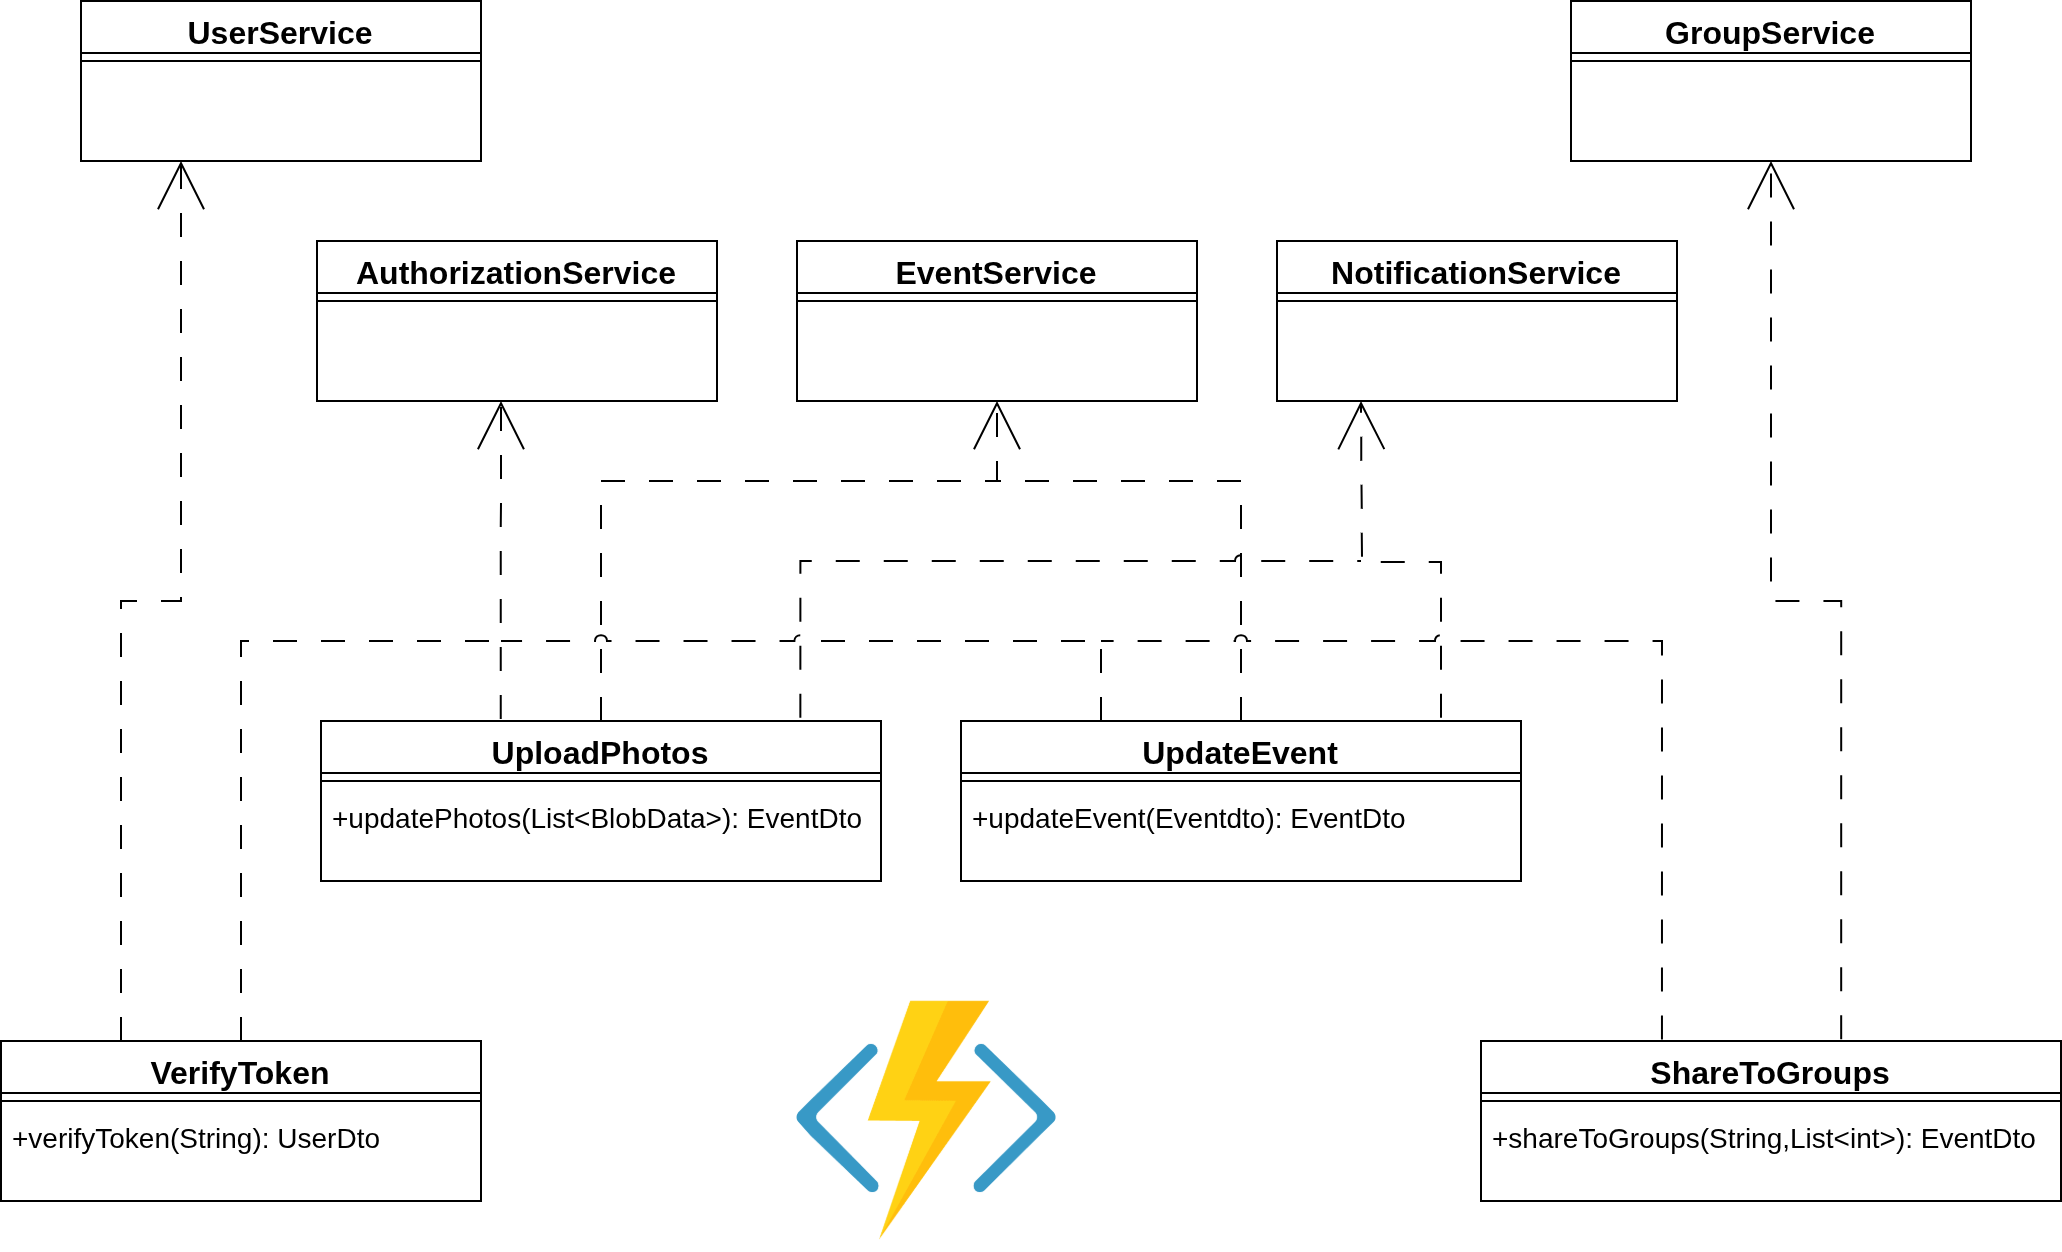
\includegraphics[width=\textwidth]{FunctionClassDiagram.png}
        \caption{Modello delle relazioni tra Functions e i servizi usati}
    \end{center}
\end{figure}

Usando la stessa modalità di suddivisione delle responsabilità
seguita per implementare l'applicativo utente,
le classi sono state sviluppate tenendo conto delle divisioni del dominio
e di ulteriori responsabilità specifiche.
Per ogni elemento principale del dominio è stata sviluppata
una classe service che implementa le operazioni relative,
mentre, per compiti che richiedono particolare attenzione o 
che astraggono l'interazione con una particolare risorsa,
vengono implementate classi apposite.\\
\clearpage
\begin{figure}[h!]
    \begin{center}
        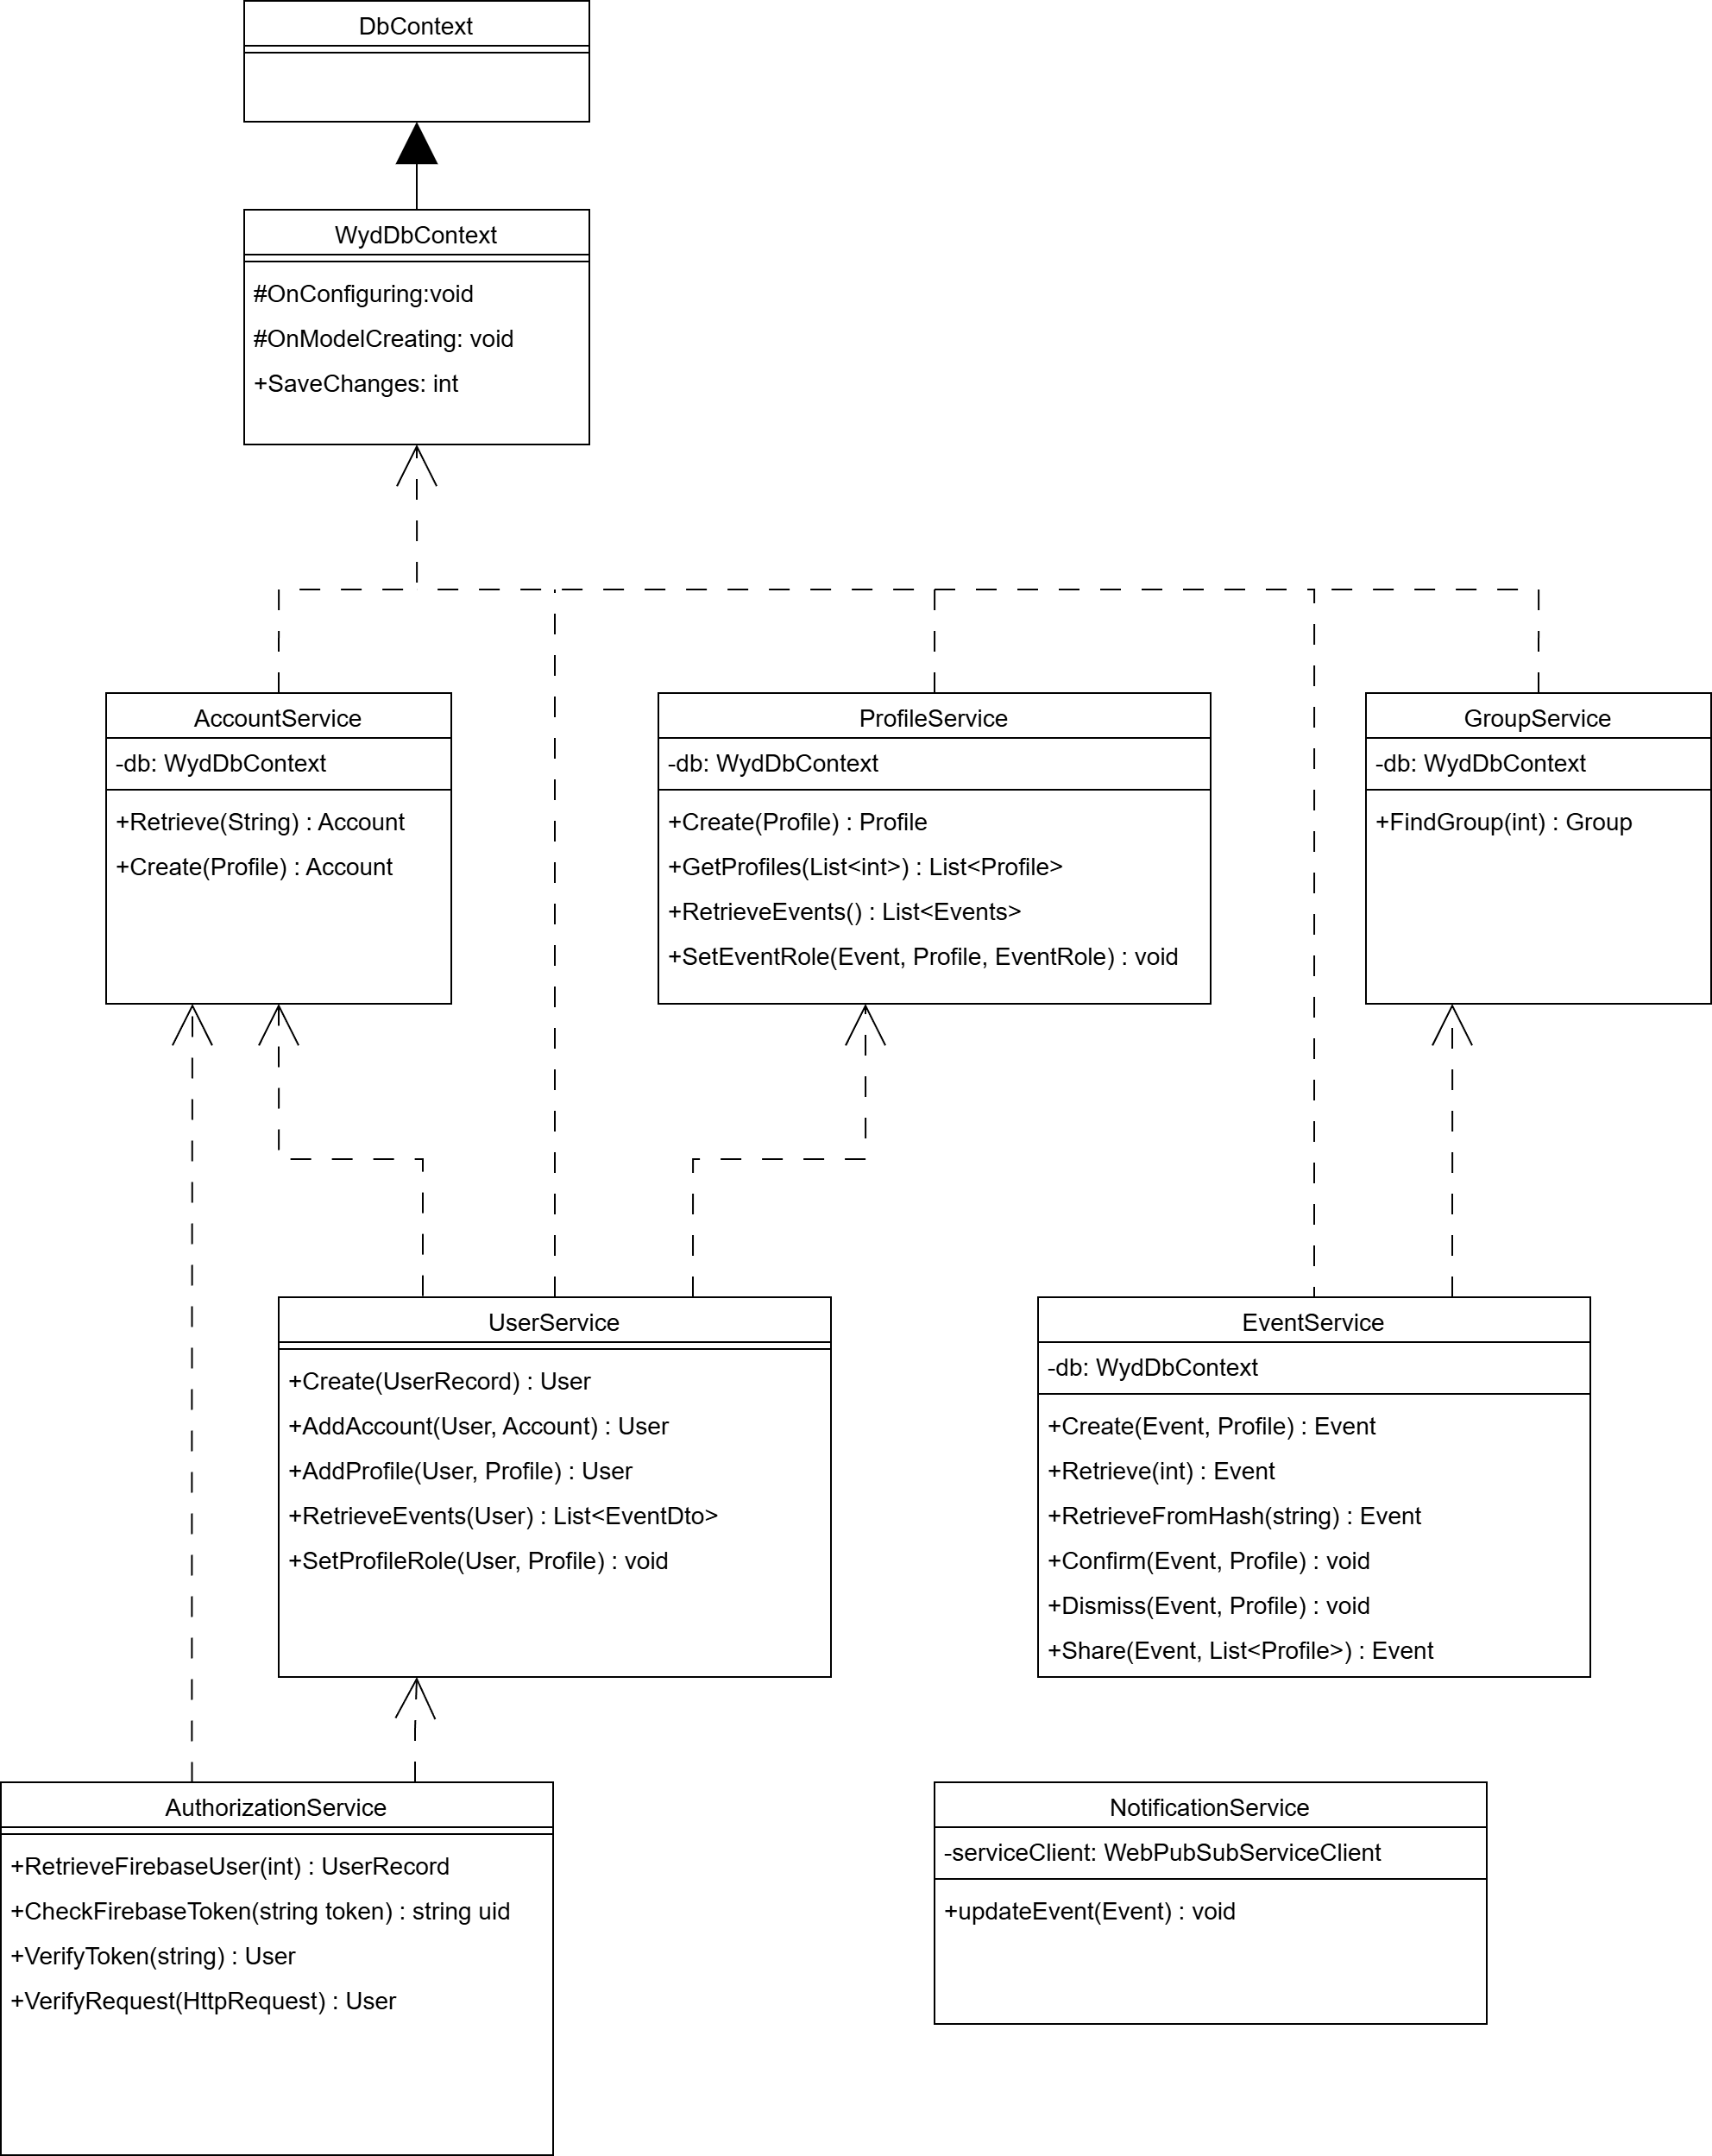
\includegraphics[height=0.8\textheight]{ServiceClassDiagram.png}
        \caption{Modello delle classi del server}
    \end{center}
\end{figure}

Ogni servizio relativo alla manipolazione degli elementi del dominio
ha bisogno di una connessione con il database
per poter applicare le modifiche desiderate.
Questa viene implementata da una classe dedicata chiamata WydDbService.
WydDbService racchiude la logica
e le impostazioni legate alla persistenza principale.
Si concentrano così in un unico luogo tutte le necessità e
le configurazioni di basso livello relative alla sua interazione,
quali la definizione del dominio e delle sue relazioni,
ma anche le proprietà degli indici e le varie operazioni,
dal recupero ad altre più particolari.
L'implementazione delle classi del dominio viene trattata nei capitoli seguenti.\\
\\
Per alcuni compiti specifici sono state implementate classi apposite.
In particolare, 
AuthorizationService si occupa dell'autenticazione e dell'autorizzazione della richiesta,
mentre NotificationService astrae la relazione 
con il servizio di aggiornamento in tempo reale.\\
\\
La maggior parte delle funzioni hanno il compito di rispondere a una richiesta REST,
in cui l'utente cerca di recuperare dei dati o di modificarli.
Ogni funzione di questo tipo seguirà in generale lo stesso procedimento.
Il primo passo consiste nell'autenticare l'utente che fa la richiesta,
analizzando il relativo token.
Si controlla poi che l'utente abbia i permessi necessari
per eseguire l'operazione desiderata.
Se è tutto in regola, si procede a elaborare i dati di ingresso
tramutandoli, se necessario, in oggetti logici.
Si procede quindi con l'esecuzione voluta, la vera responsabilità della funzione.
In base alla natura dell'operazione,
potrebbe essere opportuno aggiungere messaggi in coda per invocare altre funzioni,
quali quelle responsabili per l'invio di notifiche agli utenti coinvolti.
Infine, si restituisce la risposta dell'operazione avvenuta a buon fine,
con in allegato i dati eventualmente necessari.
Tutto il processo viene inserito in un blocco che 
permette l'identificazione di errori e la gestione della relativa risposta.\\
\\
Per allineare i dati a disposizione del server con il dominio del client
e per ridurre l'invio delle informazioni non necessarie, sono stati creati dei Data Transfer Object(DTO).
I DTO sono classi logiche che prevedono almeno un costruttore che, dato l'elemento del dominio,
ne copia solo le informazioni necessarie.
Questo permette di creare rappresentazioni dei dati come necessarie al client,
mascherando le logiche applicative e di fatto separando le dipendenze del dominio dai requisiti di comunicazione.\\
\begin{figure}[h!]
    \begin{center}
        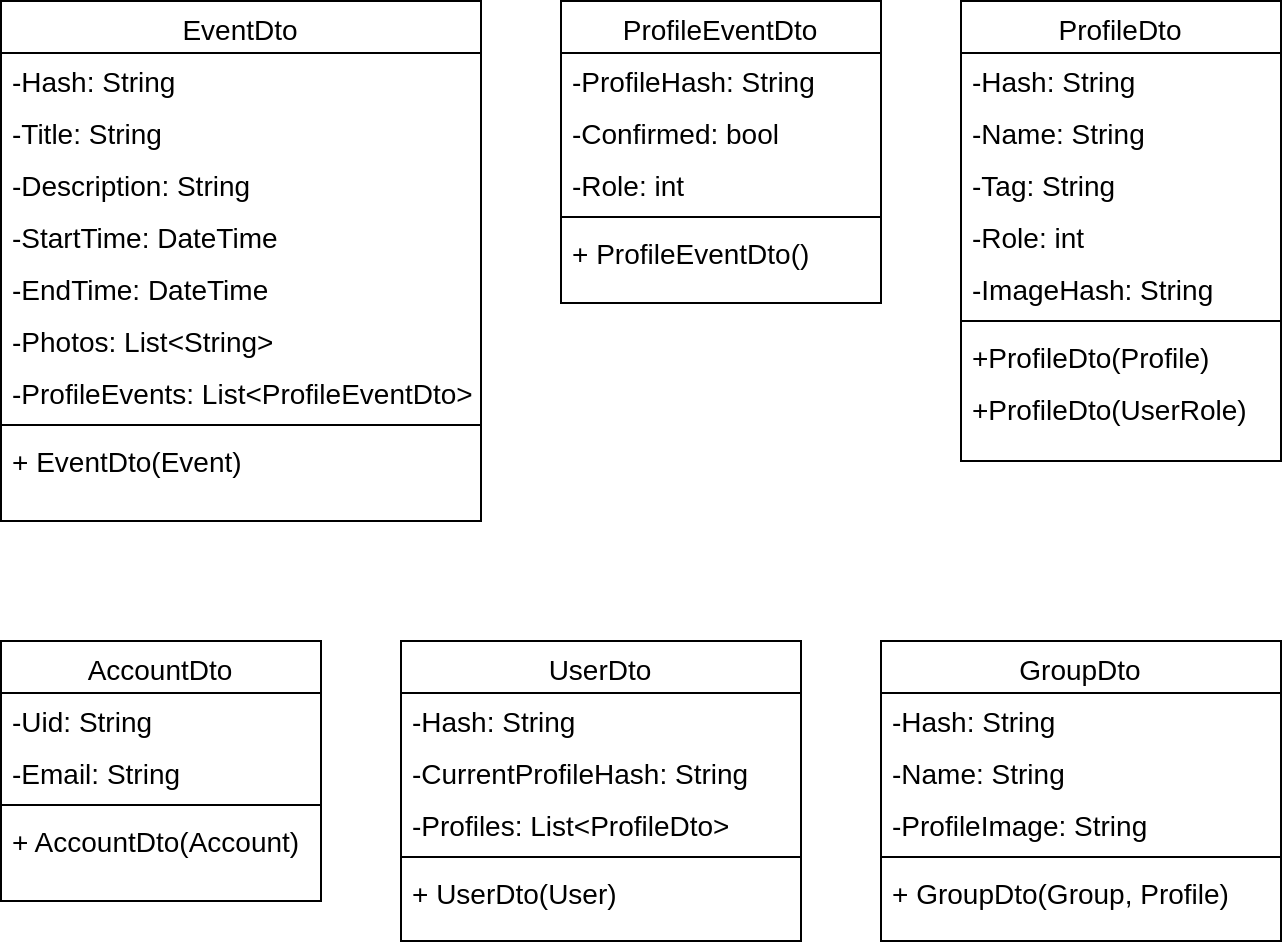
\includegraphics[width=\textwidth]{DTOClassDiagram.png}
        \caption{Modello delle classi dei data tranfer object}
    \end{center}
\end{figure}
\\
Per ogni metodo pubblico delle classi service sono stati implementati dei test.
I test permettono la simulazione di differenti situazioni
per controllare che il codice segua il comportamento desiderato.
La loro implementazione è quindi precedente allo sviluppo stesso delle classi,
in quanto le aspettative sono già note, e il superamento dei test determina la correttezza del metodo.
Inoltre, in caso di necessità particolari che escono dalle normali aspettative della funzione,
quali, ad esempio, il controllo di un valore particolare o l'implementazione di un vincolo specifico,
i test assicurano la loro futura presa in carico anche in caso di modifica totale del codice.\\
\begin{figure}[h!]
    \begin{center}
        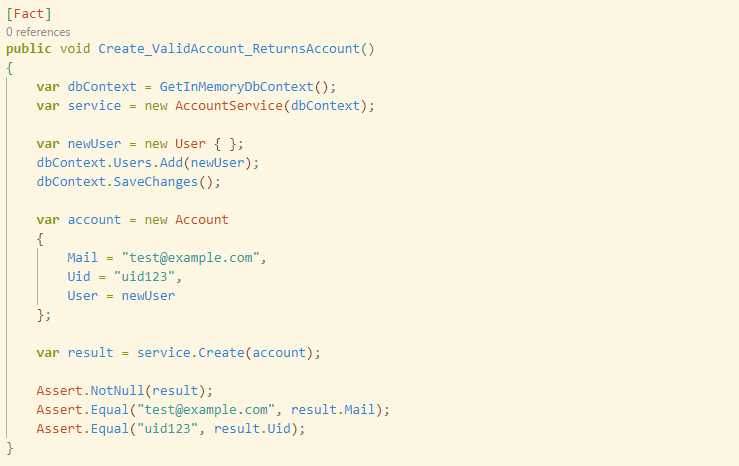
\includegraphics[height=.35\textheight]{TestAccount2.png}
        \caption{Test di creazione di un account}
    \end{center}
\end{figure}

\clearpage



